\documentclass[egilmezThesis.tex]{subfiles} 
\begin{document}


\chapter{Implementation}
\label{chap:Implementation}

Here we display the implementation of the methodology that is discussed in detail in chapter \ref{chap:example}.

Firstly we should briefly mention about the flow of the program and the structure of the input files.

The main program contains of two subprograms. The first one of those takes two input files, namely \textit{colorNames.txt} and \textit{colors.txt}.  The program takes a used-defined number of color pairs. The last two pairs are the test set, and the rest of the pairs consist the training set. One of the two pairings of the test set is expected to be from the training set, and the other one outside of the domain of the training set. So the program trains the weights via the color pairings from the training set and evaluate the credibility value of the one from the test set. For this regard, \textit{colorNames.txt} store the information concerning the names of the colors. Every line displays one pair, and in each pair colors are separated by the \textit{space} escape character. In a similar manner, in each line \textit{colors.txt} saves the \textit{RGB} values of the corresponding colors from the other input file. The six values, i.e. three for each of the colors, are separated by \textit{space} characters and lines are split with an \textit{enter key}.

An example case for the input files is displayed as follows:
\newline
\newline
\lstset{language=C++,basicstyle=\footnotesize}
\begin{lstlisting}[caption=colors.txt, breaklines=true]
250 128 114 255 127 80
255 99 71 210 105 30
154 205 50 102 205 170
178 34 34 32 178 170
220  20  60 65 105 225
255 250 250 25 25 112
255 99 71 210 105 30
255 192 203 238 130 238
\end{lstlisting}

\lstset{language=C++,basicstyle=\footnotesize}
\begin{lstlisting}[caption=colorNames.txt, breaklines=true]
Salmon Coral
Tomato Peru
YellowGreen MediumAquamarine	
FineBrick LightSeaGreen
Crimson RoyalBlue
Snow MidnightBlue
Tomato Peru
Pink Violet
\end{lstlisting}


The second subprogram works with a single input file, namely \textit{colorsAll.txt}.  The input file contains all the information regarding the complete set of colors in \textit{X11} scheme. At each line you have the name and the \textit{RGB} values of a particular color. 

The subprogram asks the user two name two colors from the domain. It then takes out those two values and their associated information from the knowledge base. All of the possible pairings between the rest of the colors are computed by the program, which exactly corresponds to $9591$ pairings. With this huge amount of information, the weights are trained and later utilized for evaluating the credibility degree of the similarity value concerning the color pairing of interest.

You may observe an example instance of the \textit{colorsAll.txt} input file. That is followed by two example outputs of the program for the same color pair, but with different methodologies of evaluating the global weight, namely \textit{minimum rule} and \textit{average rule}. And finally you may inspect the complete implementation of the methodology in \textit{C++} programming language.

\lstset{language=C++,basicstyle=\footnotesize}
\begin{lstlisting}[caption=colorsAll.txt, breaklines=true]
IndianRed 205 92 92
LightCoral 240 128 128
Salmon 250 128 114
DarkSalmon 233 150 122
LightSalmon 255 160 122
Red 255 0 0
Crimson 220 20 60
FireBrick 178 34 34
DarkRed 139 0 0
Pink 255 192 203
LightPink 255 182 193
HotPink 255 105 180
DeepPink 255  20 147
MediumVioletRed 199  21 133
PaleVioletRed 219 112 147
LightSalmon 255 160 122
Coral 255 127  80
Tomato 255  99  71
OrangeRed 255  69   0
DarkOrange 255 140   0
Orange 255 165   0
Gold 255 215   0
Yellow 255 255   0
LightYellow 255 255 224
LemonChiffon 255 250 205
LightGoldenrodYellow 250 250 210
PapayaWhip 255 239 213
Moccasin 255 228 181
PeachPuff 255 218 185
PaleGoldenrod 238 232 170
Khaki 240 230 140
DarkKhaki 189 183 107
Lavender 230 230 250
Thistle 216 191 216
Plum 221 160 221
Violet 238 130 238
Orchid 218 112 214
Fuchsia 255   0 255
Magenta 255   0 255
MediumOrchid 186  85 211
MediumPurple 147 112 219
BlueViolet 138  43 226
DarkViolet 148   0 211
DarkOrchid 153  50 204
DarkMagenta 139   0 139
Purple 128   0 128
Indigo  75   0 130
DarkSlateBlue 72  61 139
SlateBlue 106  90 205
MediumSlateBlue 123 104 238
GreenYellow 173 255  47
Chartreuse 127 255   0
LawnGreen 124 252   0
Lime 0 255   0
LimeGreen  50 205  50
PaleGreen 152 251 152
LightGreen 144 238 144
MediumSpringGreen 0 250 154
SpringGreen 0 255 127
MediumSeaGreen 60 179 113
SeaGreen 46 139  87
ForestGreen 34 139  34
Green 0 128   0
DarkGreen 0 100   0
YellowGreen 154 205  50
OliveDrab 107 142  35
Olive 128 128   0
DarkOliveGreen 85 107  47
MediumAquamarine 102 205 170
DarkSeaGreen 143 188 143
LightSeaGreen 32 178 170
DarkCyan  0 139 139
Teal  0 128 128
Aqua 0 255 255
Cyan 0 255 255
LightCyan 224 255 255
PaleTurquoise 175 238 238
Aquamarine 127 255 212
Turquoise 64 224 208
MediumTurquoise 72 209 204
DarkTurquoise 0 206 209
CadetBlue 95 158 160
SteelBlue 70 130 180
LightSteelBlue 176 196 222
PowderBlue 176 224 230
LightBlue 173 216 230
SkyBlue 135 206 235
LightSkyBlue 135 206 250
DeepSkyBlue 0 191 255
DodgerBlue 30 144 255
CornflowerBlue 100 149 237
RoyalBlue 65 105 225
Blue 0   0 255
MediumBlue 0   0 205
DarkBlue 0   0 139
Navy 0   0 128
MidnightBlue 25  25 112
Cornsilk 255 248 220
BlanchedAlmond 255 235 205
Bisque 255 228 196
NavajoWhite 255 222 173
Wheat 245 222 179
BurlyWood 222 184 135
Tan 210 180 140
RosyBrown 188 143 143
SandyBrown 244 164  96
Goldenrod 218 165  32
DarkGoldenrod 184 134  11
Peru 205 133  63
Chocolate 210 105  30
SaddleBrown 139  69  19
Sienna 160  82  45
Brown 165  42  42
Maroon 128   0   0
White 255 255 255
Snow 255 250 250
Honeydew 240 255 240
MintCream 245 255 250
Azure 240 255 255
AliceBlue 240 248 255
GhostWhite 248 248 255
WhiteSmoke 245 245 245
Seashell 255 245 238
Beige 245 245 220
OldLace 253 245 230
FloralWhite 255 250 240
Ivory 255 255 240
AntiqueWhite 250 235 215
Linen 250 240 230
LavenderBlush 255 240 245
MistyRose 255 228 225
Gainsboro 220 220 220
LightGrey 211 211 211
Silver 192 192 192
DarkGray 169 169 169
Gray 128 128 128
DimGray 105 105 105
LightSlateGray 119 136 153
SlateGray 112 128 144
DarkSlateGray  47  79  79
Black 0   0   0
\end{lstlisting}

\newpage
\begin{center}
\label{The minimum rule is utilized}
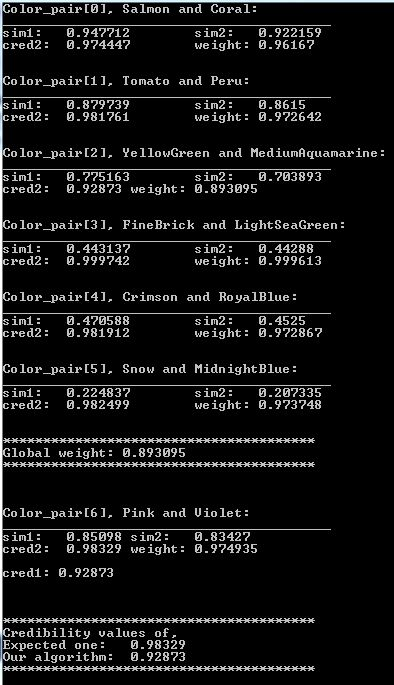
\includegraphics[width=0.8\textwidth]{2.jpg}
\end{center}

\newpage
\begin{center}
\label{The average rule is utilized}
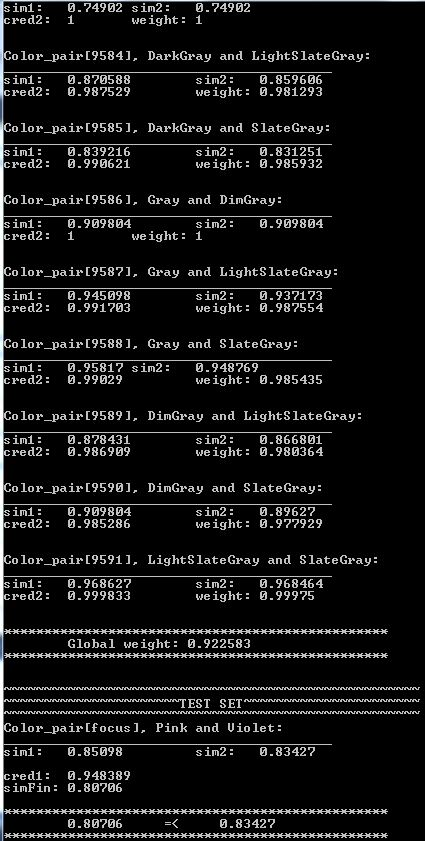
\includegraphics[width=0.8\textwidth]{3.jpg}
\end{center}

%\begin{comment}

\newpage
\lstset{language=C++,basicstyle=\footnotesize}
\begin{lstlisting}[caption=The C++ implementation of the application concerning colors, breaklines=true]

#include<iostream>
using namespace std;
#include<string>
#include<math.h>
#include <vector>
#include <string>
#include <fstream>
#include <sstream>

struct color{
	int x;			//first coordinate
	int y;			//second coordinate
	int z;			//third coordinate
	string c;		//the color name
};

float euqDist(float, float, float, float, float, float);		//euclidian distance between two colors.
float simOneColor(float, float);									//similarity between two instances of the same color.
float simByED(float);												//similarity degree of two colors via euqlidian distance.
float simByAlg(float, float, float, float, float, float);	//similarity degree of two colors via our algorithm.
float credBySim(float, float);									//credibility value defined from proximity of similarity values.
float weightEval(float, float= 1, float = (1/3.0));				//weight w, evaluated from cred function.	
float credEval(float, float= 1, float = (1/3.0));				//final credibility value, computed via global weight
void inputHandle(ifstream& f,  vector<vector<float>> &c, string fileName);
void inputColor(ifstream& f,  vector<string> &col, string fileName);
void inputComplete(ifstream& f,  vector<color> &c, string fileName);

int main()
{
	string pc;
	begin:
	cout<<"Please select your choice of program: ";
	cin>>pc;

	if(pc == "1" || pc == "A" || pc == "a"){
		ifstream f1, f2;
		vector<vector<float>> colorPairs;
		inputHandle(f1, colorPairs, "colors.txt");
		vector<string> colorNames;
		inputColor(f2, colorNames, "colorNames.txt");

		cout<<"\n~~~~~~~~~~~~~~~~~~~~~~~~~~~~~~~~~~~~~~~~~~~~~~~~~~~~\n";
		cout<<"~~~~~~~~~~~~~~~~~~~~TRAINING SET~~~~~~~~~~~~~~~~~~~~\n";
		cout<<"~~~~~~~~~~~~~~~~~~~~~~~~~~~~~~~~~~~~~~~~~~~~~~~~~~~~\n";

		float weightMin = 1;
		for(int i = 0; i < colorPairs.size() - 2; i++){
				float sim1 = simByAlg(colorPairs[i][0], colorPairs[i][1], colorPairs[i][2], colorPairs[i][3], colorPairs[i][4], colorPairs[i][5]);
				float sim2 = simByED(euqDist(colorPairs[i][0], colorPairs[i][1], colorPairs[i][2], colorPairs[i][3], colorPairs[i][4], colorPairs[i][5]));
				float cred2 = credBySim(sim1, sim2);
				float weight = weightEval(cred2);
				if(weight < weightMin)
					weightMin = weight;

				cout<<"Color_pair["<<i<<"], "<<colorNames[i*2]<<" and "<<colorNames[i*2+1]<<": "<<endl;
				cout<<"_________________________________________"<<endl;
				cout<<"sim1:\t"<<sim1<<"\tsim2:\t"<<sim2<<"\ncred2:\t"<<cred2<<" \tweight:\t"<<weight<<"\n\n\n";
		}

		cout<<"************************************************\n";
		cout<<"\tGlobal weight: "<<weightMin<<endl;
		cout<<"************************************************\n\n\n";

		cout<<"~~~~~~~~~~~~~~~~~~~~~~~~~~~~~~~~~~~~~~~~~~~~~~~~~~~~\n";
		cout<<"~~~~~~~~~~~~~~~~~~~~~~TEST SET~~~~~~~~~~~~~~~~~~~~~~\n";
		cout<<"~~~~~~~~~~~~~~~~~~~~~~~~~~~~~~~~~~~~~~~~~~~~~~~~~~~~\n";

		int s = colorPairs.size();
		for(int t = s -2; t < s; t++){
			float sim1 = simByAlg(colorPairs[t][0], colorPairs[t][1], colorPairs[t][2], colorPairs[t][3], colorPairs[t][4], colorPairs[t][5]);
			float sim2 = simByED(euqDist(colorPairs[t][0], colorPairs[t][1], colorPairs[t][2], colorPairs[t][3], colorPairs[t][4], colorPairs[t][5]));
			cout<<"Color_pair["<<t<<"], "<<colorNames[t*2]<<" and "<<colorNames[t*2+1]<<": "<<endl;
			cout<<"_________________________________________"<<endl;
			cout<<"sim1:\t"<<sim1<<" \tsim2:\t"<<sim2<<"\n\n";

			float cred1 = credEval(weightMin);	//global weight is used for finding the final credibility value
			cout<<"cred1:\t"<<cred1<<endl;
			float simFin = cred1 * sim1;
			cout<<"simFin:\t"<<simFin;

			cout<<"\n\n************************************************\n";
			cout<<"\t"<<simFin<<"     =<     "<<sim2<<endl;
			cout<<"************************************************\n\n\n";
		}
	}

	else if(pc == "2" || pc == "B" || pc == "b"){
		ifstream f3;
		vector<color> col;
		inputComplete(f3, col, "colorsAll.txt");
		string userColor1, userColor2;

		cout<<"\nPlease choose two colors: ";
		cin>>userColor1;
		cin>>userColor2;

		color temp1, temp2;
		for(int i = 0; i < col.size(); i++){
			if(col[i].c == userColor1){
				temp1.c = col[i].c;				//store the color at a temp variable
				temp1.x = col[i].x;
				temp1.y = col[i].y;
				temp1.z = col[i].z;

				col[i].c = col[col.size()-1].c;	//switch it with the last element of
				col[i].x = col[col.size()-1].x;	//the vector in order to pop it out
				col[i].y = col[col.size()-1].y;	//of the list
				col[i].z = col[col.size()-1].z;
				col.pop_back();
			}
		}

		for(int i = 0; i < col.size(); i++){
			if(col[i].c == userColor2){
				temp2.c = col[i].c;				//store the color at a temp variable
				temp2.x = col[i].x;
				temp2.y = col[i].y;
				temp2.z = col[i].z;

				col[i].c = col[col.size()-1].c;	//switch it with the last element of
				col[i].x = col[col.size()-1].x;	//the vector in order to pop it out
				col[i].y = col[col.size()-1].y;	//of the list
				col[i].z = col[col.size()-1].z;
				col.pop_back();
			}
		}

		cout<<"\n Weights evaluated via Min or Average rule: ";
		cin>>pc;

		float weightGlo = 1.0;		//global weight
		if(pc == "1" || pc == "m" || pc == "M"){
			color t1, t2;
			int pn =1;					//pair counter

			for(int i = 0; i < col.size(); i++){
				for(int j = i+1; j < col.size(); j++){
					float sim1 = simByAlg(col[i].x, col[i].y, col[i].z, col[j].x, col[j].y, col[j].z);
					float sim2 = simByED(euqDist(col[i].x, col[i].y, col[i].z, col[j].x, col[j].y, col[j].z));
					float cred2 = credBySim(sim1, sim2);
					float weight = weightEval(cred2);
					if(weight < weightGlo)
						weightGlo = weight;

					cout<<"Color_pair["<<pn<<"], "<<col[i].c<<" and "<<col[j].c<<": "<<endl;
					cout<<"_________________________________________"<<endl;
					cout<<"sim1:\t"<<sim1<<"\tsim2:\t"<<sim2<<"\ncred2:\t"<<cred2<<" \tweight:\t"<<weight<<"\n\n\n";
					pn++;
				}
			}
		}

		else if(pc == "a" || pc == "A" || pc == "2"){
			color t1, t2;
			vector<float> weights;
			int pn =1;					//pair counter
			for(int i = 0; i < col.size(); i++){
				for(int j = i+1; j < col.size(); j++){
					float sim1 = simByAlg(col[i].x, col[i].y, col[i].z, col[j].x, col[j].y, col[j].z);
					float sim2 = simByED(euqDist(col[i].x, col[i].y, col[i].z, col[j].x, col[j].y, col[j].z));
					float cred2 = credBySim(sim1, sim2);
					float weight = weightEval(cred2);
					weights.push_back(weight);

					cout<<"Color_pair["<<pn<<"], "<<col[i].c<<" and "<<col[j].c<<": "<<endl;
					cout<<"_________________________________________"<<endl;
					cout<<"sim1:\t"<<sim1<<"\tsim2:\t"<<sim2<<"\ncred2:\t"<<cred2<<" \tweight:\t"<<weight<<"\n\n\n";
					pn++;
				}
			}
			for(int i = 0; i < col.size(); i++)
				weightGlo += weights[i];
			weightGlo /= col.size();
		}

		cout<<"************************************************\n";
		cout<<"\tGlobal weight: "<<weightGlo<<endl;
		cout<<"************************************************\n\n\n";

		cout<<"~~~~~~~~~~~~~~~~~~~~~~~~~~~~~~~~~~~~~~~~~~~~~~~~~~~~\n";
		cout<<"~~~~~~~~~~~~~~~~~~~~~~TEST SET~~~~~~~~~~~~~~~~~~~~~~\n";
		cout<<"~~~~~~~~~~~~~~~~~~~~~~~~~~~~~~~~~~~~~~~~~~~~~~~~~~~~\n";

		float sim1 = simByAlg(temp1.x, temp1.y, temp1.z, temp2.x, temp2.y, temp2.z);
		float sim2 = simByED(euqDist(temp1.x, temp1.y, temp1.z, temp2.x, temp2.y, temp2.z));
		cout<<"Color_pair[focus], "<<temp1.c<<" and "<<temp2.c<<": "<<endl;
		cout<<"_________________________________________"<<endl;
		cout<<"sim1:\t"<<sim1<<" \tsim2:\t"<<sim2<<"\n\n";

		float cred1 = credEval(weightGlo);	//global weight is used for finding the final credibility value
		cout<<"cred1:\t"<<cred1<<endl;
		float simFin = cred1 * sim1;
		cout<<"simFin:\t"<<simFin;

		cout<<"\n\n************************************************\n";
		cout<<"\t"<<simFin<<"     =<     "<<sim2<<endl;
		cout<<"************************************************\n\n\n";
	}

	else{
		cout<<"Wrong command!\n";
		goto begin;
	}

	getchar();
	getchar();
	return 0;
}

//euclidian distance between two colors
float euqDist(float a, float b, float c, float x, float y, float z)
{
	return sqrt(pow(fabs(a-x),2)+pow(fabs(b-y),2)+pow(fabs(c-z),2));
}

//similarity between two instances of the same color. (ex: red_90 and red_187)
float simOneColor(float c1, float c2)
{
	return 1-((fabs(c1-c2))/255);
}

//similarity degree of two colors via euqlidian distance
float simByED(float dist)
{
	return 1-(dist/(255*sqrt(3.0)));
	/*
	float res = 1-(dist/(255*sqrt(3.0)));
	if(res < 0.1)
		return 0;
	else
		return res;*/
}

//similarity degree of two colors via our algorithm
float simByAlg(float a, float b, float c, float x, float y, float z)
{
	return (((simOneColor(a, x))+(simOneColor(b, y))+(simOneColor(c, z)))/3);
}

//credibility value defined from proximity of similarity values
float credBySim(float sim1, float sim2)
{
	//return 1-(fabs(sim1 - sim2));
	float sim = (sim2+0.01) / (sim1+0.01); 	//in order to prevent division by zero
	if(sim > 1)
		return 1;
	else 
		return sim;
}

//weight w, evaluated from cred function
float weightEval(float cred, float va, float ea)				//default values for va and ea are 1 and 1/3 respectively
{																	//since those are the most common cases, but could be overwritten
	return ((cred-ea)/(va-ea));
}

float credEval(float weight, float va, float ea)				//again default values for va and ea are 1 and 1/3 respectively
{
	return ((weight * va) + ((1-weight) * ea));
}


void inputHandle(ifstream& f,  vector<vector<float>> &c, string fileName)
{
	string temp;
	f.open(fileName);

	if (!f) {
	cout << "Unable to open file";
	cin>>temp;
	exit(1); // terminate with error
	}

	int i = 0;
	char line[1024];


	while(f.getline(line, 1024)){
		istringstream ss(line, istringstream::in);
		float rate;
		vector<float> temp;

		c.push_back(temp);

		for(int j = 0; j < 6; j++){
			ss >> rate;
			c[i].push_back(rate);
		}
		i++;
	}

	f.close();
}

void inputColor(ifstream& f,  vector<string> &c, string fileName)
{
	string temp;
	f.open(fileName);

	if (!f) {
	cout << "Unable to open file";
	cin>>temp;
	exit(1); // terminate with error
	}

	char line[1024];
	string tempColor;

	while(f.getline(line, 1024)){
		istringstream ss(line, istringstream::in);
		ss >> tempColor;				//first color of the pairing
		c.push_back(tempColor);
		ss >> tempColor;				//second color of the pairing
		c.push_back(tempColor);
	}

	f.close();
}

void inputComplete(ifstream& f,  vector<color> &c, string fileName)
{
	string temp;
	f.open(fileName);

	if (!f) {
	cout << "Unable to open file";
	cin>>temp;
	exit(1); // terminate with error
	}

	char line[1024];

	while(f.getline(line, 1024)){
		istringstream ss(line, istringstream::in);
		color temp;

		ss >> temp.c;
		ss >> temp.x;
		ss >> temp.y;
		ss >> temp.z;

		c.push_back(temp);

		cout<<temp.x<<" \t"<<temp.y<<" \t"<<temp.z<<" \t"<<temp.c<<endl;
	}

	f.close();
}

\end{lstlisting}

%\end{comment}



\end{document}